\subsection{Software Design Considerations}

\todo{remove notes}
(10, 2100 w)

Has the student clearly described the design of their system? Is it described
in sufficient detail to make it easy for someone else to replicate the system?

Has the student justified the design decisions, and discussed alternatives that
were considered?


\subsection{Architecture} 
\label{sec:design:architecture}

\begin{figure}
  \begin{center}
    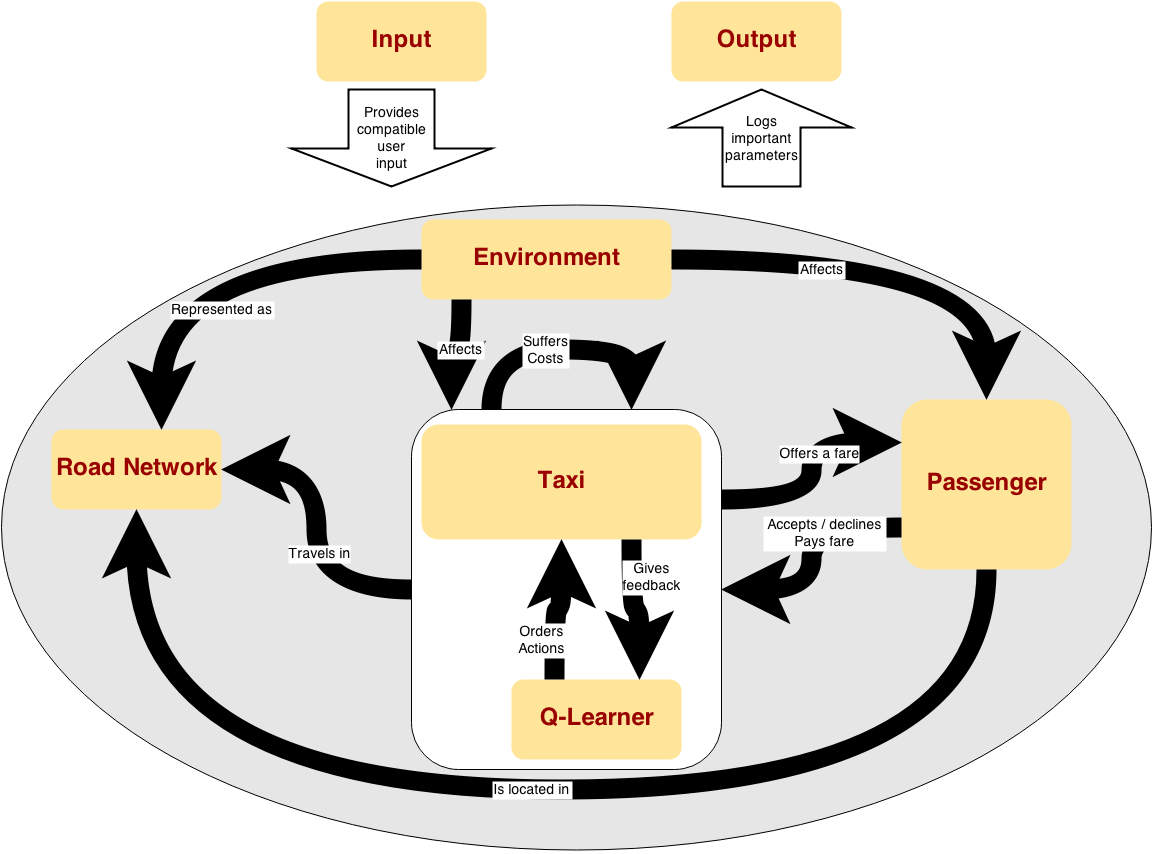
\includegraphics[width=\textwidth]{../figures/software_overview}
    \caption{
      Software overview diagram
      \label{figure:design:software}
    }
  \end{center}
\end{figure}

A software overview diagram is shown in Figure \ref{figure:design:software}.
This section explains the diagram and how the software operates.

When running the simulation, initially some user inputs are processed by the
input module. It validates that the input data (initially parsed from files or
command line parameters) is correct, stopping the program and warning the user
if any invalid data was found. The rest of the system is then initialised
according to the parameters, and a simulation is started.

The environment module is the highest hierarchy simulation object where all
other objects operate in. It is used for keeping track of global variables such
as time and the road network. The environment can directly affect the taxi and
passengers, setting their parameters, and taxis can query the environment for
some information.

The road network is internally represented as a graph, and is where taxis and
passengers are located and interact in.

Passengers (passive agents) can accept or decline taxis' offers respective to
their internal state. If accepted, passengers travel with the taxi in the road
network and pay the agreed fare. Regardless of the action taken, passengers
disappear after any action is completed.

Taxi (an active agent) is the most complex object in the software. Over time
taxi experiences its own costs (fixed costs and variable costs). Taxis can take
three types of actions: wait at a location, drive to a different location, or
offer a fare to a passenger (if one is present). Taxi's actions are decided by
its learner module. The taxi passes information from the environment to the
learner and receives calls to action. For example, the learner needs to know
what prices it can set (from taxi itself or the environment), what locations it
can drive to (from the road network), whether there is a passenger at the
current location (from the environment), what the passenger's answer to the
offer was (from the passenger).

Finally, there is an output module that logs simulation data to files for
analysis.


\subsection{Technologies}

One of the core technologies used was \textit{git} \parencite{Git} version
control software. Git when used in conjunction with \textit{GitHub}
\parencite{Github} enabled easy code backups to be hosted safely online.
Besides this, commit messages were aimed to be descriptive so that they serve
as a form of documentation of programmer's intentions.

The rest of the technologies used for this project form distinct groups and are
described in the following sections.

\subsubsection{Programming Language}

\textit{Ruby} programming language was chosen as the core technology for this
project due to author's familiarity with it and its related technologies. Ruby
is an object-oriented "dynamic, open source programming language with a focus
on simplicity and productivity. It has an elegant syntax that is natural to
read and easy to write" \parencite{Ruby}.

Ruby has many open-source libraries called \textit{gems} available, hosted and
managed locally by \textit{rubygems} software \parencite{Rubygems}. As these
gems have different versions and dependencies, they need to be managed on a
per-application basis - this process is made easy by \textit{bundler}
\parencite{Bundler}. More on these tools can be found in the Maintenance Manual
in Appendix \ref{sec:maintenance_manual}.

\subsubsection{Cross-Platform Operation and Automation}

Managing different Ruby versions on a single computer can be cumbersome in case
it is needed for multiple Ruby applications. Furthermore, Ruby development for
Windows operating systems (OS) is several months behind development on 
Unix-based systems \parencite{Ruby}, rendering the latest versions of Ruby unusable
directly on Windows, which also happens to be the case with this project.

Fortunately, this can easily be avoided by using the following software:
\textit{VirtualBox} \parencite{Virtualbox} virtualisation software to host any
of the most popular OSs, \textit{Vagrant} \parencite{Vagrant} to automatically
manage the OSs and software installed on them, and \textit{RVM} \parencite{Rvm}
to manage Ruby versions on a single OS. Detailed instructions on using this
software stack with Ruby are in the Maintenance Manual in Appendix
\ref{sec:maintenance_manual}. This method also means that the programmer can
easily move between computers as the setup costs are significantly reduced by
automation.


\subsubsection{Supporting Test-Driven Development}
\label{sec:design:software:tdd}

As was explained in Section \ref{sec:design:tdd}, Test-Driven Development (TDD)
is an important method for software development in this project. Therefore
supporting effective TDD is critical. \textit{RSpec} is a TDD testing tool for
Ruby \parencite{Rspec}. The tests describe the desired behaviour of software in
a domain-specific language aimed to be very close to natural English.

An example RSpec test scenario is shown in Figure \ref{figure:rspec}. This test
specifies behaviour of some ruby class 'Class' which should have a 'currency'
method that returns 'EURO'. If multiple tests are written specifying the
expected behaviour in different conditions, then RSpec tests become a form of
programmer-friendly documentation that is executable and protects the code from
introducing regression bugs.

\begin{figure}
  \begin{verbatim}
    describe Class do
      describe '#currency' do
        it 'is EURO' do
          instance = Class.new
          expect(instance.currency).to eq('EURO')
        end
      end
    end
  \end{verbatim}
  \caption{
    RSpec test example
    \label{figure:rspec}
  }
\end{figure}

RSpec can be enhanced by other tools. \textit{Simplecov} \parencite{Simplecov}
is a code coverage tool that monitors test coverage of a codebase by checking
how many lines of code are executed when running the test suite. \textit{Guard}
\parencite{Guard} is a tool that monitors file changes and executes appropriate
events (i.e. running RSpec tests). This can make a developer's TDD work flow
streamlined leaving the developer with only tests and code to write.
